\subsection{Current Sensor}
The Current Sensor must measure the current from the Generator in order to protect the Load System from electrical overload. The Current Sensor is built using a Hall-effect based current transducer of the type LTS 15-NP\cite{CurrentTransducer}. This type of transducer was also used in the Power Sensor design. Like before, the transducer is configured in such a way that it is able to measure currents up to $\SI{48}{\ampere}$ with a accuracy of 0.2\%.

The Current Sensor is able to measure currents in the range of $\pm \SI{48}{\ampere}$. This range is simply chosen out of simplicity since this was the same as earlier. This range is bigger than what it must be as a $\SI{15}{\ampere}$ fuse is implemented in series with the sensor.

\begin{figure}[H]
	\centering
	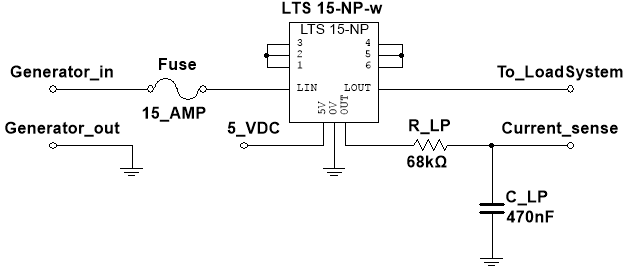
\includegraphics[width=0.8\linewidth]{Hardware/LoadSystem/CurrentSensor}
	\caption{Configuration of Current Sensor in the system}
	\label{fig:CurrentSensorCircuit}
\end{figure}

As the transducer is tested during the Power Sensor's unity test in section \vref{sec:PowerSensorTest}. During this test it was found that the output-volt can be calculated exactly as it is specified in the datasheet:
\begin{equation}
	V_{out} = 2.5 + \left( 0.625 \cdot \frac{I_{in}}{\SI{15}{\ampere}}\right)
\end{equation}